\documentclass[12pt]{article}

\usepackage[utf8]{inputenc}
\usepackage[T1]{fontenc}
\usepackage{a4}
\usepackage{lipsum}
\usepackage{graphicx}
\usepackage{float}
\usepackage{listings}
\usepackage{color}
\usepackage{cite}
\usepackage{textgreek}
\usepackage{amsfonts}
\usepackage{enumitem}

\usepackage[margin=1in]{geometry}

\definecolor{dkgreen}{rgb}{0,0.6,0}
\definecolor{gray}{rgb}{0.5,0.5,0.5}
\definecolor{mauve}{rgb}{0.58,0,0.82}

\lstset{frame=tb,
  language=matlab,
  aboveskip=5mm,
  belowskip=5mm,
  showstringspaces=false,
  columns=flexible,
  basicstyle={\small\ttfamily},
  numberstyle=\tiny\color{gray},
  keywordstyle=\color{blue},
  commentstyle=\color{dkgreen},
  stringstyle=\color{mauve},
  breaklines=true,
  breakatwhitespace=true,
  tabsize=2
}

\title{
  {\Huge \bf Power Systems Lab}\\
  \vspace{0.25in}

  {\bf Experiment 8}\\
  Laboratory Report
  \vspace{1in}
}
\author{
  \bf Syed Alisamar Husain, 17BEE012\\
  B.Tech Electrical Engg, 8th Semester
}

\begin{document}
  \begin{titlepage}
    \maketitle
    \vspace*{\fill}
    \begin{center}
      {\bfseries Department of Electrical Engineering} \\
      Jamia Millia Islamia, New Delhi
    \end{center}
    \thispagestyle{empty}
  \end{titlepage}
  
  \newpage
  \begin{center}
    \huge Experiment 8
    \vspace{0.5in}
  \end{center}

  \section{Objective}
  Develop a simulink model for the single phase 
  energization of a 3-phase transmission line.

  {\bf Let the given problem be as follows:}
  \begin{center}
    \it
    A 250 km, three-phase line is energized on a 100 kV network. 
    The line is first energized on phase A at t = 1/4 cycle 
    (maximum of source voltage). Phase B and phase C are left open. 
    Find the transients on the moment of switching.
  \end{center}

  \section{Theoretical Background}
    \subsection{Long Transmission Line}
    {\bf A long transmission line} is defined formally as a power transmission 
    line with an effective {\bf length more than 120 km}. 
    Unlike short transmission lines and medium transmission lines, 
    it is no longer reasonable to assume that the line parameters 
    are lumped. 

    {\bf In a long transmission line the line constants are uniformly 
    distributed over the entire length of line.} This is because the 
    effective circuit length is much higher than what it was for the 
    former models (long and medium line) and hence we can no longer 
    ignore the shunt admittance of the line and 
    ignore the mutual inductance of the line.

    \subsection{Switching Transients in Circuit Breakers}
    {\bf Switching transients occur in power systems each time an abrupt circuit 
    change occurs.} These transients are short lived and oscillatory in nature. 

    In a typical switching operation, such as a contactor or breaker 
    opening or closing, switching transients occur on an electrical load 
    each time an abrupt circuit change, or current chop, occurs.
    When the two breaker contacts separate, an arc is created in the 
    interrupter that maintains current flow. 
    \begin{figure}[H]
      \centering
      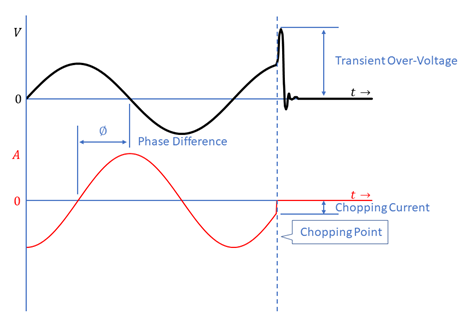
\includegraphics[width=3in]{img/switching-transient-graph.png}
    \end{figure}

  \pagebreak
  \section{Implementation}
  The model is implementated by using the {\bf distributed parameters line and the
  long line Pi-model} in the Simscape Electrical library of Simulink.
  A {\bf single-phase voltage source} is connected via a source impedance to a 
  circuit breaker. 
  
  {\bf The line is energized by the closing of this circuit breaker.}
  As breaker closes at 1/4th of the cycle, it produces a {\bf transient current}. 
  When the breaker contacts join, an arc is created in the 
  interrupter that maintains current flow. As the current approaches its next 
  zero-crossing, the arc weakens then extinguishes. 

  Switchings are performed simultaneously on two different line models:
  \begin{enumerate}[label=\Alph*]
    \item. Distributed Parameters Line
    \item. Pi-model Parameters Line
  \end{enumerate}

  \begin{figure}[H]
    \centering
    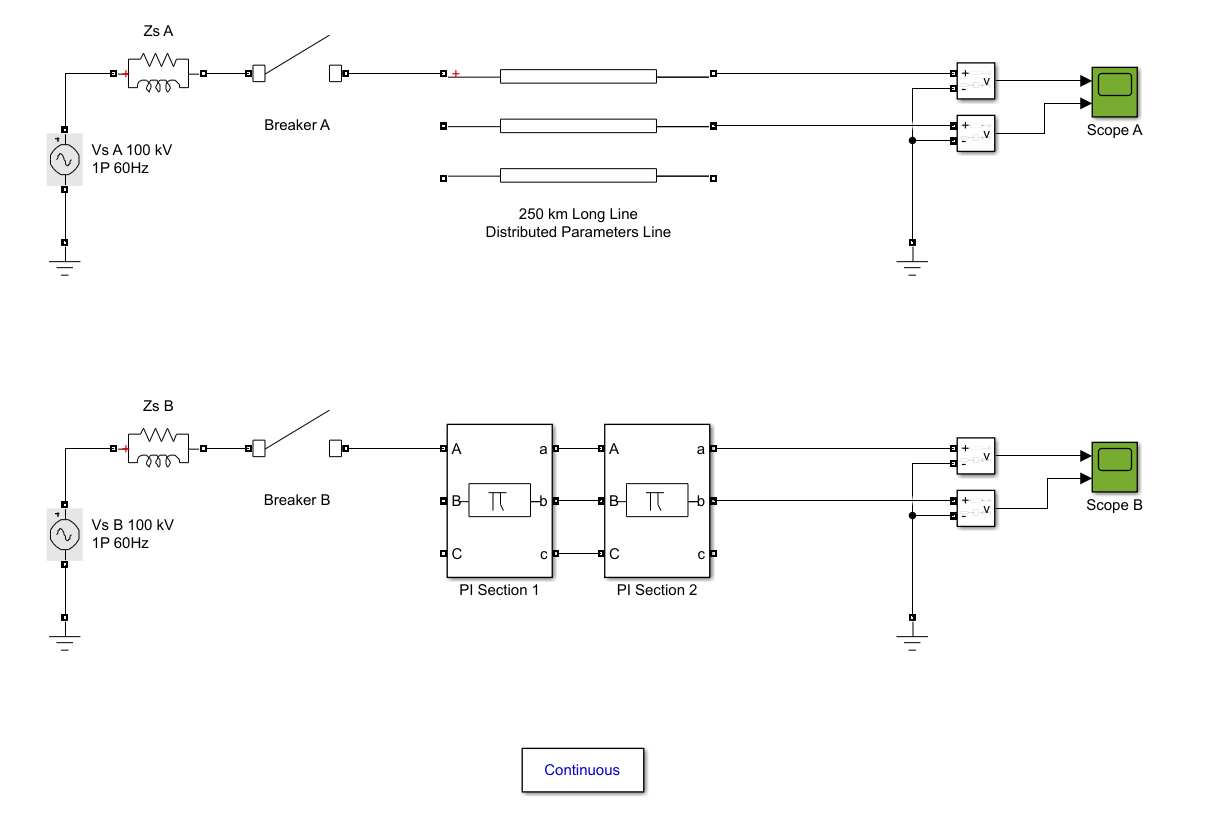
\includegraphics[width=6in]{img/model.png}
    \caption{Simulink Model Implementation}
    \label{Model}
  \end{figure}

  For both of these models, {\bf we measure the voltage on the recieving end} 
  between the phase A to Ground, as well as phase B to Ground.

  \pagebreak
  \section{Observations}
  For both of the transmission line models, we measured the voltage on the 
  recieving end between the phase A to Ground, as well as phase B to Ground.

    \subsection{Distributed Parameters Line}
    At the moment of switching the {\bf phase voltage increases to 137.3 kV peak} and
    oscillates at the system frequency. {\bf This lasts for 400 ms,} and
    the {\bf voltage settles at 103.2 kV.}
    \begin{figure}[H]
      \centering
      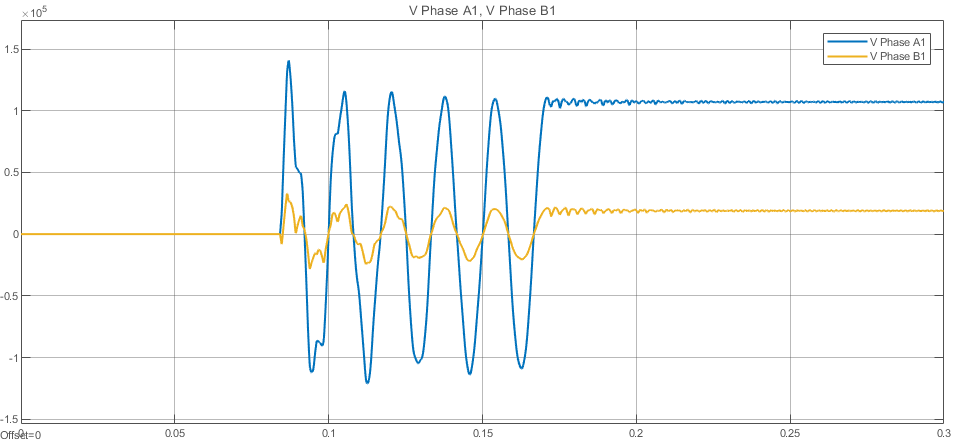
\includegraphics[width=5in]{img/scope_a.png}
      \caption{Distributed Parameters Line}
      \label{scope_a}
    \end{figure}


    \subsection{Pi-model Parameters Line}
    At the moment of switching the {\bf phase voltage increases to 139.7 kV peak} and
    oscillates at the system frequency. {\bf This lasts for 430 ms,} and
    the {\bf voltage settles at 110.5 kV.}
    \begin{figure}[H]
      \centering
      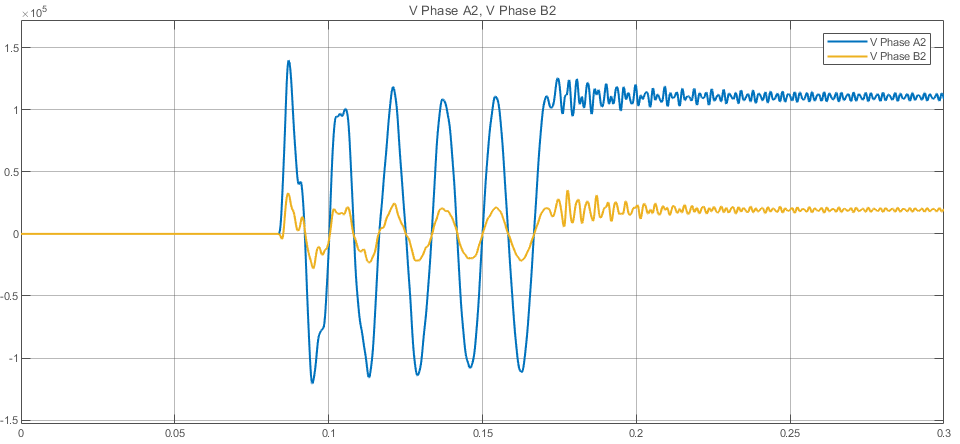
\includegraphics[width=5in]{img/scope_b.png}
      \caption{Pi-model Parameters Line}
      \label{scope_b}
    \end{figure}
  
  We also observe that in both cases, there is a voltage induced in phase B which
  follows the oscillation of phase A and {\bf rises to a peak of 32.4 kV.}

  \section{Result}
  We observed the single phase energization transients in a 3-phase transmission
  line with two line models.
  We also observed that in both cases, there is a voltage induced in the adjacent
  phase which follows the oscillation of the energized phase.

\end{document}